\chapter{Appendix A}\label{Further Results}

\section{Building Energy Analysis}
\label{s:buildingResults}
	
	The optimal configurations of the ASF can be visualised using carpet-plots. For a classical building analysis this was done for every hour of the year. Figures \ref{f:DIVAx} and \ref{f:DIVAy} show the optimizing altitude and azimuth angles for heating, cooling, lighting and total building energy demand. In figure \ref{f:DIVAx}, darker colours represent closed positions, whereas brighter colours correspond to open positions. To optimize heating and lighting, open positions (corresponding to large altitude angles) are favourable, cooling is optimized by using closed positions (corresponding to small altitude angles). The overall optimized solutions follow the corresponding patterns at the hours of importance. The azimuth angles in figure \ref{f:DIVAy} correspond to the deviation from the facade normal. For a south facing facade, this means an angle with a positive sign represents the panels facing towards south-east (bright colours), whereas negative angles represent the panels facing towards south-west (dark colours). It can be seen that for heating and lighting, the facade takes positions that let the sun in, whereas for cooling the facade follows a sun-tracking pattern which prevents radiation to enter the room. 

	\begin{figure*}
		\begin{center}
		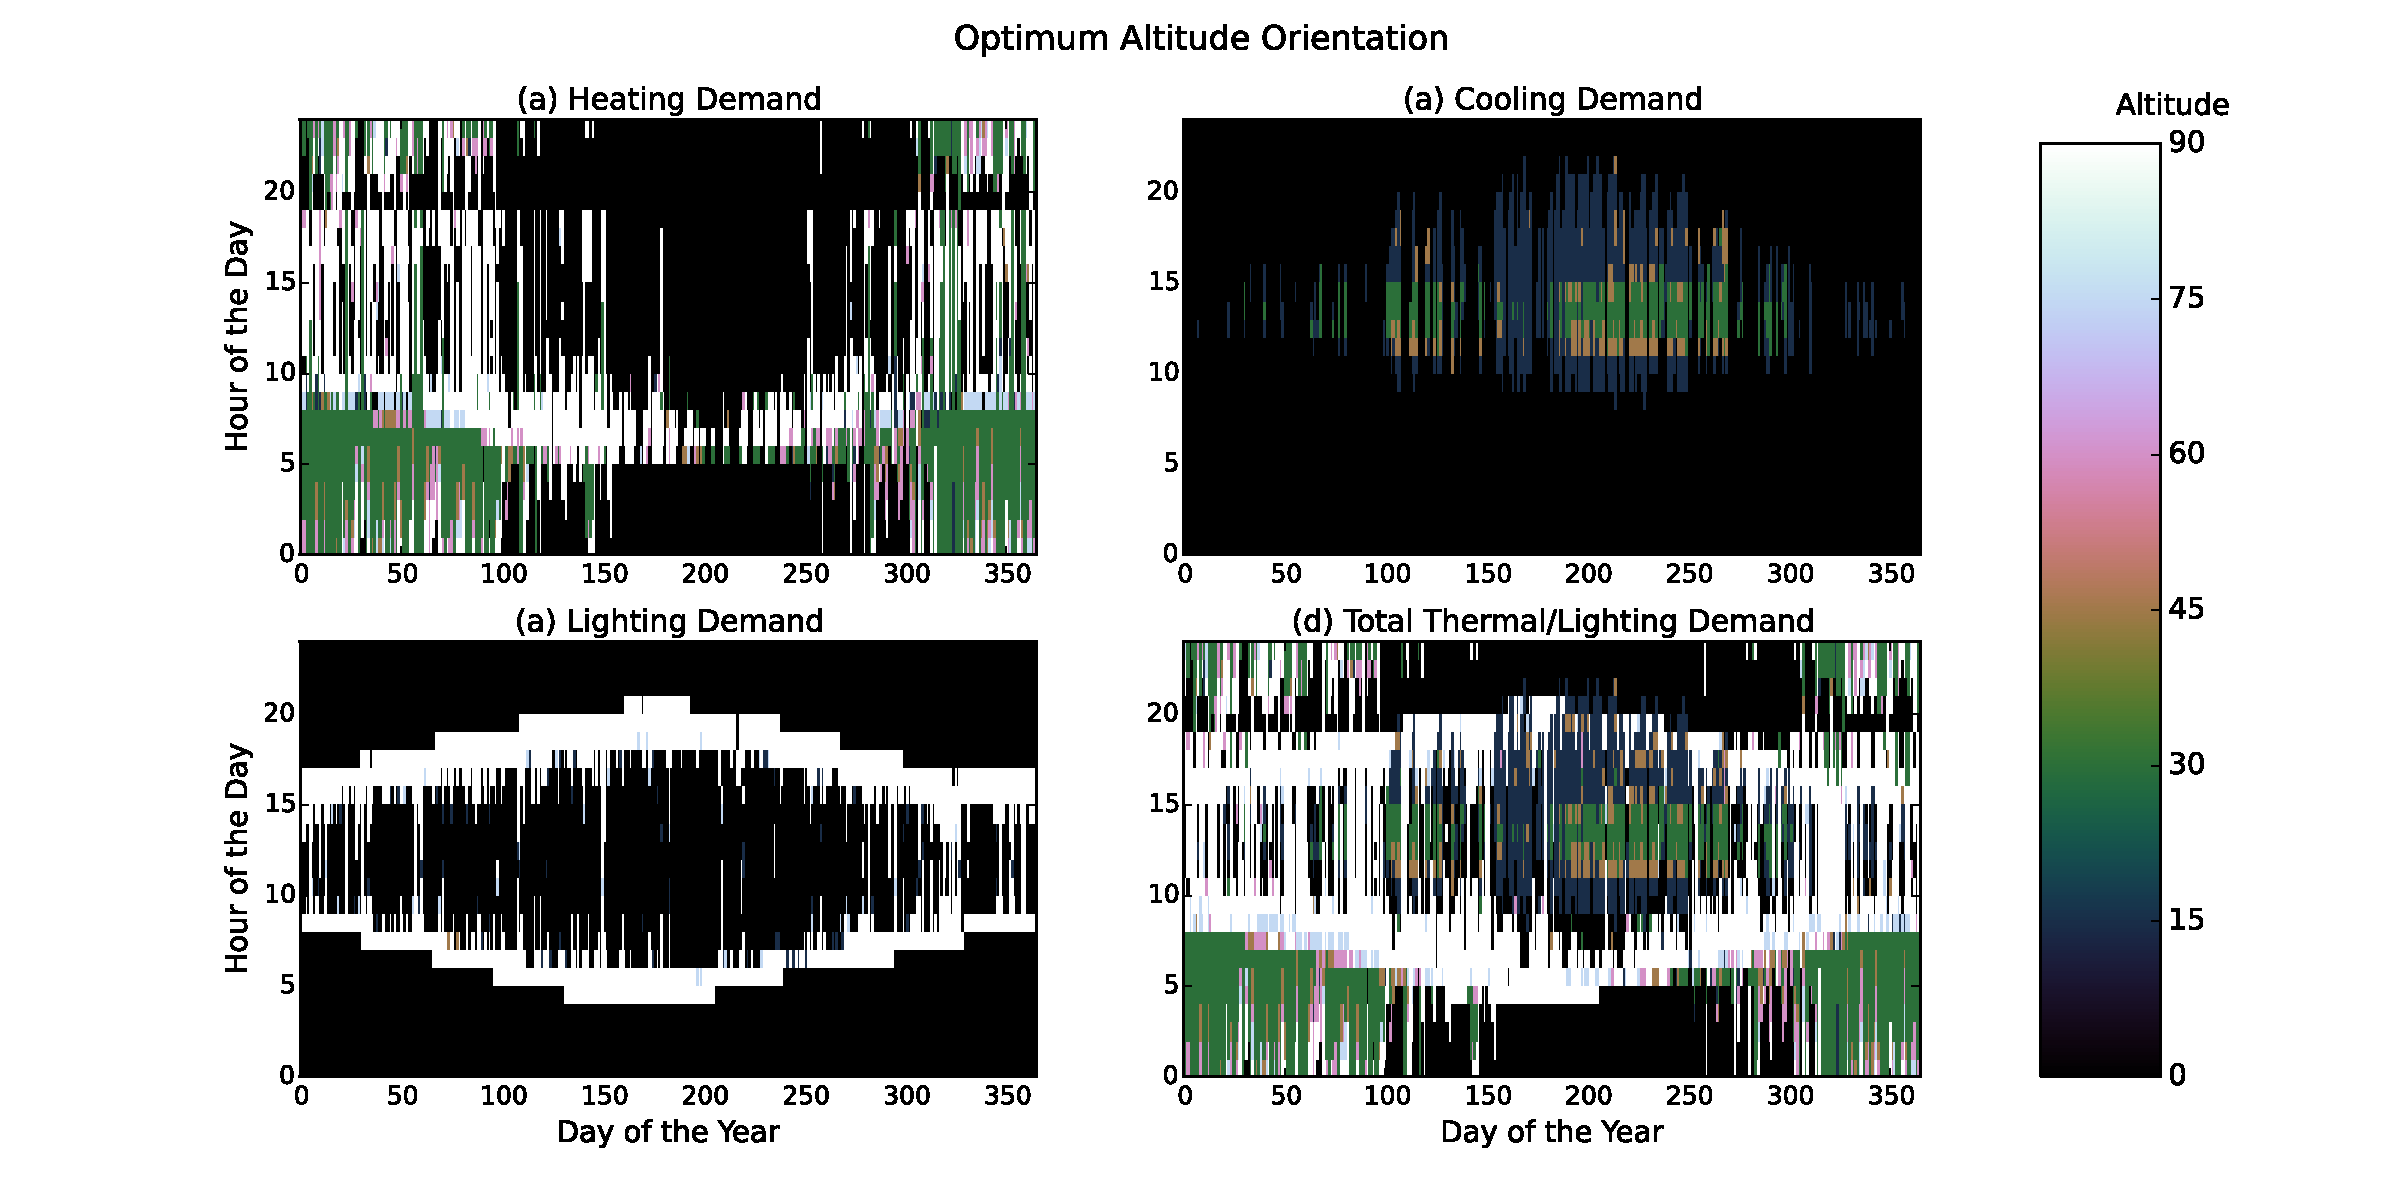
\includegraphics[width=\textwidth, trim= 0cm 0cm 0cm 0cm,clip]{DIVAx}
		\caption{Carpet plots detailing the optimal altitude angles to minimise the (a) heating demand, (b) cooling demand, (c) lighting demand, and (d) total building energy demand. Darker colours represent closed positions, whereas brighter colors correspond to open positions. To optimize heating and lighting, open positions are favorable, cooling is optimized by using closed positions.}
		\label{f:DIVAx}
		\end{center}
	\end{figure*}


	\begin{figure*}
		\begin{center}
		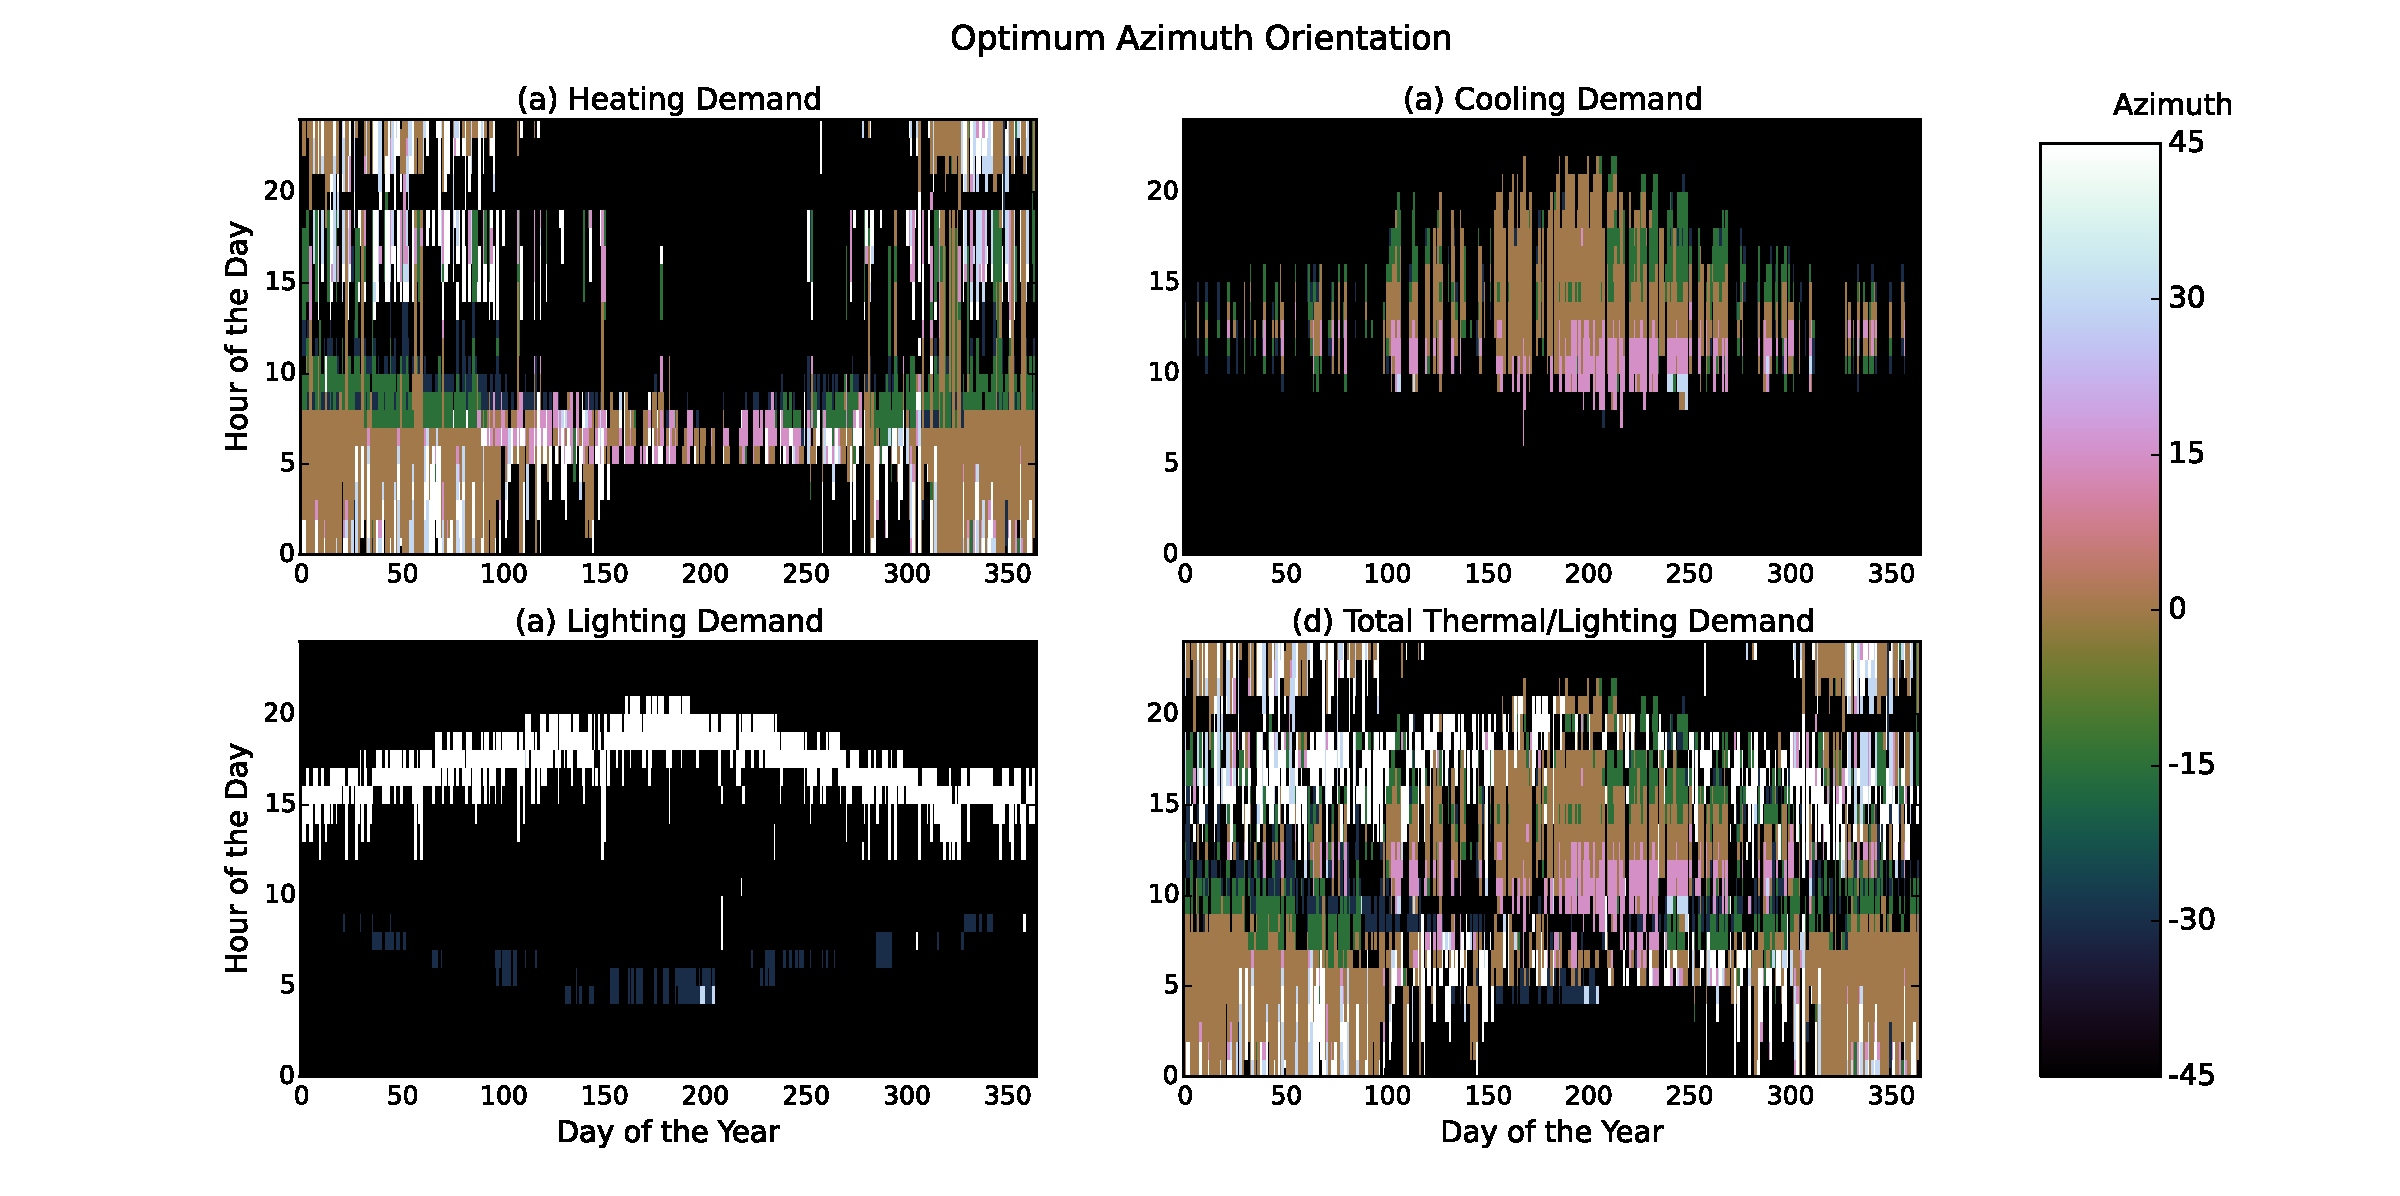
\includegraphics[width=\textwidth, trim= 0cm 0cm 0cm 0cm,clip]{DIVAy}
		\caption{Carpet plots detailing the optimal azimuth angles to minimise the (a) heating demand, (b) cooling demand, (c) lighting demand, and (d) total building energy demand. Cooling is minimized by bocking the sun, whereas lighting and heating is minimized by opening the facade to let the insolation in.}
		\label{f:DIVAy}
		\end{center}
	\end{figure*}

	Figure \ref{f:DIVAe} depicts the corresponding energy demand of the building for the whole year corresponding to the optimum positions presented in figures \ref{f:DIVAx} and \ref{f:DIVAy}. It can be seen that the heating heating is most needed during the winter and in the morning, whereas cooling is mainly apparent in summer afternoons. Lighting on the other hand is most important in the evenings and at times where there is not much sun. In the combined plot, this behavior be seen clearly as well, the main overlaps of different building energy consumptions take place during winter between heating and lighting in the morning and in the evening, and between cooling and lighting during summer evenings. 

	\begin{figure*}
		\begin{center}
		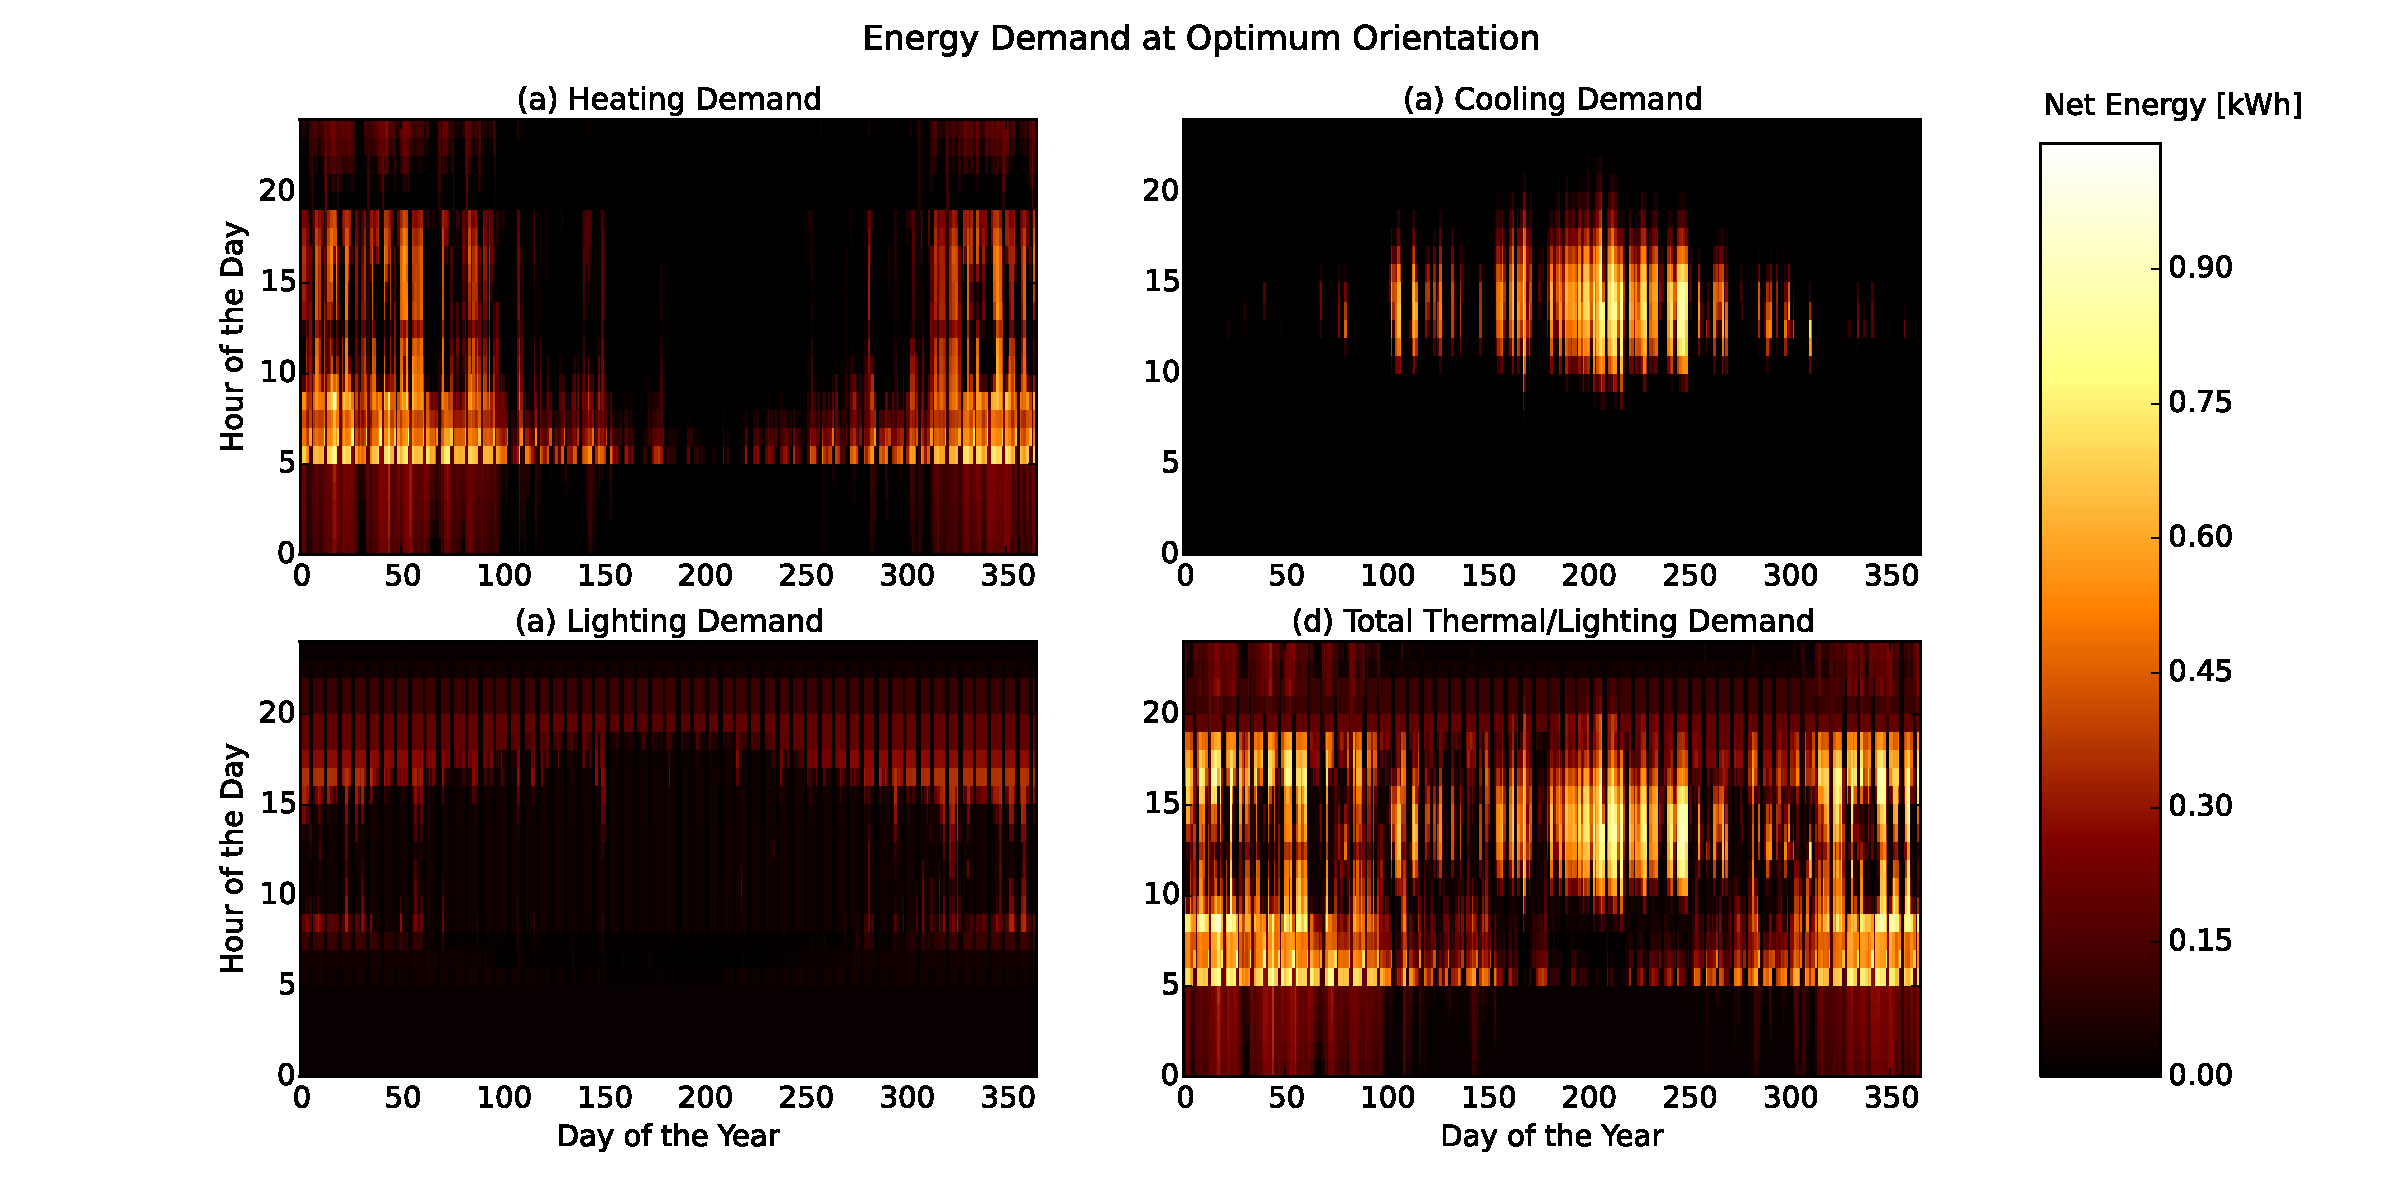
\includegraphics[width=\textwidth, trim= 0cm 0cm 0cm 0cm,clip]{DIVAe}
		\caption{Carpet plots detailing the net energy consumption. Each square represents the total energy consumption for that specific hour of the entire month. Red colours detail the energy demand, while blue colours detail the energy supply.}
		\label{f:DIVAe}
		\end{center}
	\end{figure*}
	
	
	
	
	
	